\documentclass{beamer}

\usefonttheme[onlymath]{serif}
\usepackage{subfig}
\usepackage{amsmath}
\usepackage{mathtools}

\title{Distributed Laplacian Solver}
\author{Rahul V}

\begin{document}

%1
\frame {
    \titlepage
}

%2
\frame {
    \frametitle{Problem Statement: Solve Lx = b}
    \begin{itemize}
        \item
            $x^{T}L=b^{T}$
        \item
            Laplacian matrix: $L = D - A$
        \item
            Adjacency matrix: $A_{uv} = w_{uv}$
        \item
            Diagonal matrix: $D_{uu} = \sum_{v=1}^{v=n}A_{uv}$
        \item
            One sink: $b_{n} = -\sum_{i=1}^{n-1}b_{i}$
    \end{itemize}
}

%3
\frame {
    \frametitle{Algorithm}
    \begin{itemize}

        \item
            Solve Data Collection Problem (DCP)
            \begin{itemize}
                \item[\textbullet]
                    Each node generates a packet with probability $\beta J_{u}$
                \item[\textbullet]
                    Transmit a packet to a random neighbor $v$ with
                    probability $w_{uv}$
                \item[\textbullet]
                    Packets sunk at the sink immediately
            \end{itemize}
        \item
            Let $\eta$ be the queue occupancy probability at
            stationarity
        \item
            $\eta^{T}(I - P) = \beta J^{T}$
            or
            $(\eta^{T}D^{-1})L = \beta J^{T}$

    \end{itemize}
}

%4
\frame {
    \frametitle{Results}
    \framesubtitle{Dense graphs}
    \begin{itemize}
        \item $N\_PROC = 4$
        \item Randomly generated graphs
        \item Spielman's solver employs Cholesky factorization
    \end{itemize}
    \begin{figure}
        \centering
        \subfloat[Performance]{
            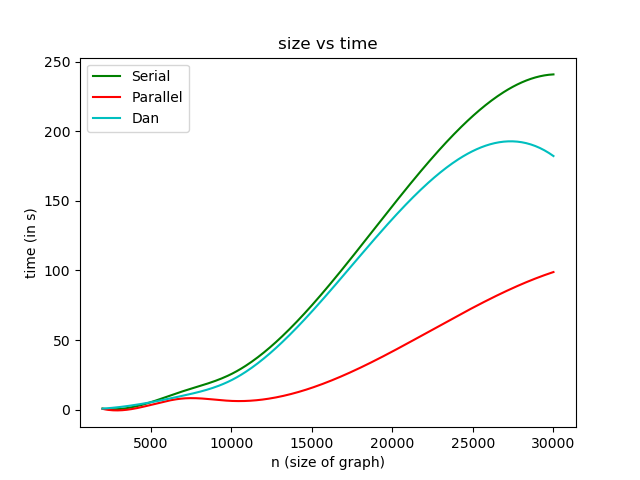
\includegraphics[height=5cm,width=7cm]{img/dense.png}
        }
        \label{fig:plots}
    \end{figure}
}

%5
\frame {
    \frametitle{Results}
    \framesubtitle{Sparse graphs}
    \begin{itemize}
        \item
            Terribly slow, in contrast to the Spielman's blazing fast solver
            \\
            (27s vs 0.34s)
        \item
            Reason:
            \begin{itemize}
                \item[\textbullet]
                    Most solvers exploit sparsity; running time
                    is linear in $\#edges$
                \item[\textbullet]
                    ALG relies on fraction of packets sunk ($C$)
                \item[\textbullet]
                    Random path to sink is longer in sparse graphs
            \end{itemize}
        \item
            Solution:
            \begin{itemize}
                \item[\textbullet]
                    Move the packets $k$ steps at a time (Densify)
                \item[\textbullet]
                    Each packet can move to any node within k hops
            \end{itemize}
    \end{itemize}
}

%6
\frame {
    \frametitle{Result of k-step speed-up}
    \framesubtitle{Sparse graphs}
    \begin{figure}
        \centering
        \subfloat[Speed up]{
            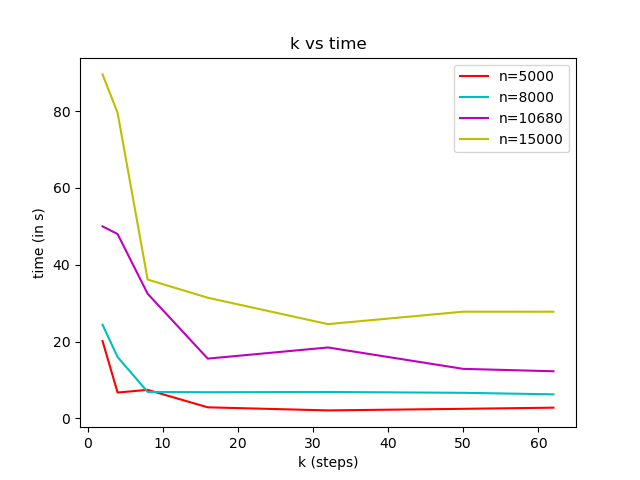
\includegraphics[height=6cm,width=8cm]{img/k.png}
        }
        %\subfloat[Performance]{
        %    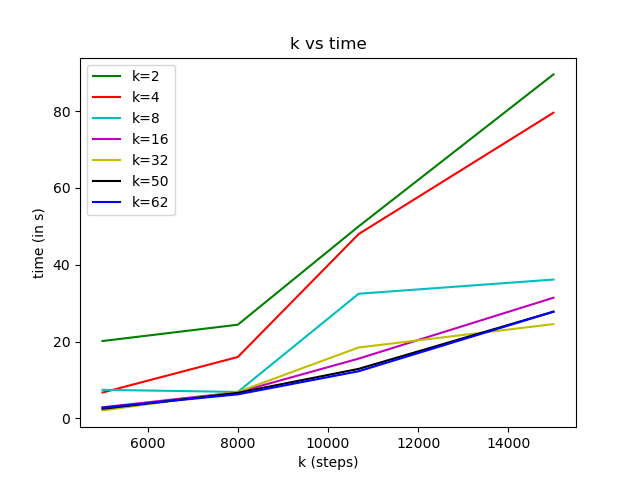
\includegraphics[height=4cm,width=5cm]{img/nk.png}
        %}
        \label{fig:speed}
    \end{figure}
}

%7
\frame {
    \frametitle{Approximation of an approximate solution}
    \begin{itemize}
        \item
            No speedup on dense graphs
        \item
            Satisfies a slightly different relation at stationarity
        \begin{itemize}
            \item[\textbullet]
                $\eta^{T}(I - P^{k}) = k\beta J^{T}$
        \end{itemize}
        \item
            Retreiving original solution, $\alpha$, without speed up:
        \begin{itemize}
            \setlength\itemsep{0.5em}
            \item[\textbullet]
                $\eta^{T}(I - P^{k}) = k\alpha^{T}(I - P)$
            \item[\textbullet]
                $\alpha^{T} = \eta^{T}(I + P + \dots + P^{k-1})/k$
        \end{itemize}

        \item
            ALG performs just as good for sparse graphs now
    \end{itemize}
}

%8
\frame {
    \frametitle{Other algorithms of interest}
    \begin{itemize}
        \item
            Becchetti's algorithm:
        \begin{itemize}
            \setlength\itemsep{0.5em}
            \item[\textbullet]
                Send out \emph{all} packets in each round
            \item[\textbullet]
                The $|Q_{u}|$ (not $\eta_{u}$) itself would be the
                solution.
            \item[\textbullet]
                $Q(t+1) = Q(t)P + \beta J$
            \item[\textbullet]
                $\#rounds$ to converge is lesser but time taken is more
            \item[\textbullet]
                Overall, performs worse than ALG
            \item[\textbullet]
                Unfortunately, the k step speed up doesn't help in this
                case.
        \end{itemize}
    \end{itemize}
}

%4
%\frame {
%    \frametitle{Status quo: Practical concerns}
%    \framesubtitle{Testing}
%    \begin{itemize}
%        \item
%            Guarantee by the algorithm:\\
%            $|x_{u} - \hat{x_{u}}| < (\epsilon_{1} + \epsilon_{2})x_{u}$
%            , whenever $\kappa < x_{u}d_{u}$
%        \item
%            Test set construction:
%            \begin{itemize}
%                \item[\textbullet]
%                    $m =$ random from $[n - 1, n(n - 1)/2]$
%                \item[\textbullet]
%                    Generate Random MST with random weights in $[0, 100]$
%                \item[\textbullet]
%                    Generate random edges by selecting $2$ random nodes
%                \item[\textbullet]
%                    $b_{i}$ is chosen randomly from $[0, 1000]$
%            \end{itemize}
%    \end{itemize}
%}

%5
%\frame {
%    \frametitle{Status quo: Practical concerns}
%    \framesubtitle{Performance}
%    \begin{itemize}
%        \item
%            $(\kappa, \epsilon_{1}, \epsilon_{2}) = (0.1, 0.1, 0.1)$
%        \item
%            Shared memory model with $4$ threads
%        \item
%            Fixed number of rounds ($O(nlogn)$), sampling from the start
%    \end{itemize}

%    %\begin{figure}
%    %    \centering
%    %    \subfloat[Performance]{
%    %        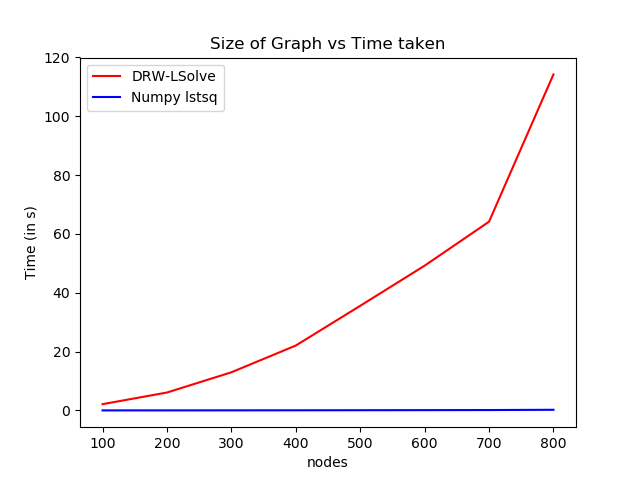
\includegraphics[height=5cm,width=5cm]{img/tcomp.png}
%    %    }
%    %    \subfloat[Accuracy]{
%    %        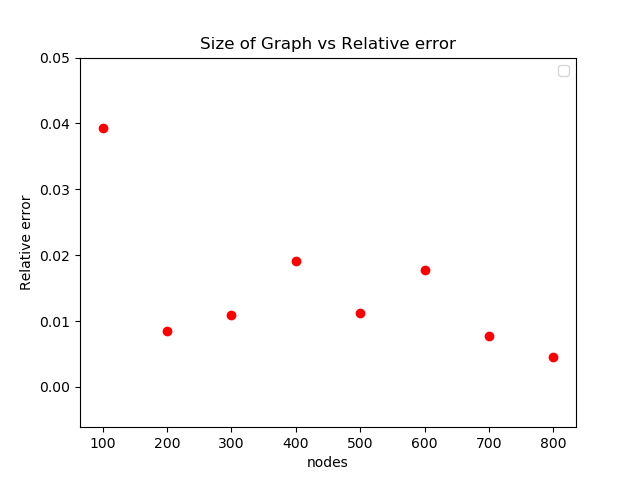
\includegraphics[height=5cm,width=5cm]{img/relerr.png}
%    %    }
%    %    \label{fig:plots}
%    %\end{figure}

%}

%6
%\frame {
%    \frametitle{Near future}
%    \begin{itemize}
%        \item
%            Use Message Passing instead of Shared memory model
%        \item
%            Graph partitioning to reduce communications, who should be at the
%            boundary:
%            \begin{itemize}
%                \item[\textbullet]
%                    Work as long as possible without need for checking queue
%                \item[\textbullet]
%                    Get very few packets in the first place
%            \end{itemize}
%    \end{itemize}
%}

%7
\frame[c] {
    \centering \Huge \emph{Thank you}
}

\end{document}
